\documentclass[10pt,twoside]{article}
\usepackage{graphicx}
\usepackage{url}
\usepackage{hyperref}
\usepackage{multirow}
\hypersetup{
	colorlinks=true,
	citecolor=blue,%
    filecolor=blue,%
    linkcolor=blue,%
    urlcolor=blue
}

\newcommand{\doctitle}{%
Graph Coloring}
\newcommand{\cmnt}[1]{}

\pagestyle{myheadings}
\markboth{\hfill\doctitle}{\doctitle\hfill}

\bibliographystyle{siam}

\addtolength{\textwidth}{1.00in}
\addtolength{\textheight}{1.00in}
\addtolength{\evensidemargin}{-1.00in}
\addtolength{\oddsidemargin}{-0.00in}
\addtolength{\topmargin}{-.50in}

\hyphenation{in-de-pen-dent}

%\title{\textbf{\doctitle}\\
\title{\textbf{Graph Coloring Using State Space Search}}

\author{Sandeep Dasgupta\thanks{Electronic address: \texttt{sdasgup3@illinois.edu}}
\qquad Tanmay Gangwani\thanks{Electronic address: \texttt{gangwan2@illinois.edu}}
\qquad Mengjia Yan\thanks{Electronic address: \texttt{mengjia@illinois.edu}}
\qquad  Novi Singh \thanks{Electronic address: \texttt{novi.singh94@gmail.com}}} 

\begin{document}

\thispagestyle{empty}

\maketitle
\section{Introduction}
As a subject with many applications, graph coloring is one of the most studied
  NP-hard problems. Due to its time complexity graph coloring is an excellent
  candidate for implementation with a parallelized architecture, and as such
  has become our choice for our project. Of the many ways that graph coloring
  can be adapted for parallel programming there are two main approaches in
  literature: the iterative and state-space search methods.  The iterative
  approach begins by dividing the vertices of the graph to be colored into
  different groups, each of which is assigned to a node in the parallelized
  system. In the context of Charm++ this would be akin to dividing the vertices
  among a set of chares. At this point each chare would independently color its
  assigned vertices, and once all vertices had been colored the chares would
  communicate with each other to see if each of their respective vertices had
  any neighbors on other chares that violate the constraints of the coloring
  problem. Once color conflicts have been assessed the chares would seek to
  mediate these problems through another round of independent coloring among
  the chares, a process that would be repeated until the graph has been
  successfully colored or shown to be uncolorable for a number of colors. 

  Unlike the iterative approach, state-space seeks to start with the initial
  graph and color it by creating child chares for each possible color
  assignment among the vertices. This process of coloration and child creation
  is repeated until a solution to the coloring problem is found or an
  exhaustive search has yielded no solution. By doing so the program explores
  all different possible colorations of the graph for a number of colors.
  State-space search has an advantage over the iterative approach in that it
  does not require the large number of messages sent by the method’s chares to
  mediate coloring conflicts, nor does it have to deal with the complexity of
  mediation caused by highly connected subgraphs in the main graph. However,
            the state-space search does require the use of many more chares
              than the iterative approach and in doing so occurs higher memory
              overhead. In our opinion the message usage of the iterative
              approach outweights the memory footprint of the state-space.
              Additionally, we chose to focus on finding the first solution
              given a user provided maximum of  colors, k. Once found we keep on
              decrementing k untill the graph become uncolorable. With this
              we can achieve the optimal  coloring under the heristics applied.
              
\section{.ci file structure}
Our implementation of state-space search is outlined in the structure of our
  .ci file. At the start of the program a root node is created by the main
  chare. This chare is responsible for graph preprocessing, namely
  precoloration, vertex removal, and independent subgraph detection (all will
      be discussed shortly). After preprocessing, the root selects a vertex to
  color, using a heuristic, and then spawns child nodes(chares) for each
  possible coloring of that vertex following a ordering based on another
  heuristic (called value ordering to be discussed later) and  provides them with information regarding what has been colored
  already, and then waits for their response.  The children of the root, and
  all subsequently created child nodes, also begin by preprocessing the graph,
      but only vertex removal and independent subgraph detection are applied.
        The response can be a success or failure and based on that the child
        states are merged with the parent to create an  updated response which
        is propagated up to its parent. Each merge node has the intelligence to
        prune of redundant searches. For example, if a node which has spawned
        chares for independent graphs figures out that one of its subgraph is
        returning ``failure of coloring'', then it ensures the the other
        subgraphs need not to be explored. 
  
  Grain size is the determining factor of the next step, causing the child to
  either spawn child nodes with value ordering if a determining factor is
  greater than the grain size, or to sequentially color the graph if it is
  equal to or less than it. 

      Chares are additionally grouped together, and result signals from the
      leaf nodes of the search are given higher privilege via the expedited
      tag. In doing so the problem of kill-chasing, that is the ineffective
      signaling of the end of the program due to competing the forces of “kill”
      messages and the spawning of new chares, is addressed.

\section{Heuristics for State-Space Search}
Due to the NP-hard nature of the problem the number of all possible states in
  the state-space search is exponential in size, and as such heuristics to
  reduce the number of states that are searched are necessary for any tractable
  computation to be possible. Some of the ideas are borrowed from
  \cite{Kale1995}.

\begin{itemize}  
  \item \textbf{Pre-Coloring} \\
  The first of these heuristics is a preprocessing technique, namely the
  precoloring of the graph. By finding the 3-cliques in the graph we are able
  to preemptively assign them colors before the primary coloring algorithm
  begins. However, due to the extremely interconnected nature of dense graphs
  with large numbers of vertices, this technique is best applied to sparse
  graphs. As dense graphs tend to have many, many 3-cliques, this preprocessing
  technique often results in an almost entirely sequential coloring of the
  graph, may end up reporting un-colorability of the graph even though it is
  colorable. This is because the underlying algorithm to color is too naive,
    i.e. to put any possible color to a vertex such that it does not interfere
      with its neighbors.

  \item \textbf{Variable Ordering (Selecting a vertex to color next)} \\
            An intuitive and simple heuristic guides our process for selecting
            the next vertex to be colored. By picking the vertex with the least
            available number of potential colors we can more effectively move
            throughout the graph providing a likely path towards the solution. 
            This pairs well with our next pair of heuristics which are \textbf{impossibility
            testing} and \textbf{forced move} testing respectively. In the former, if
            after a vertex is colored if one of its neighbors has 0 available
            colors then the state for that coloring is not generated. The
            latter dictates that if the number of colors of the neighbor is
            brought down to 1, then the neighbor should be colored in that same
            step. This process is repeated recursively as well as coloring a
            neighbor might lead to another forced-move for its neighbor.  
            
  \item \textbf{Vertex Removal} \\
            The next applicable heuristic is vertex removal. By noting that a
            vertex with degree less than the number of available colors must
            always have a valid possible coloring, we can remove such a vertex
            from the graph (pushing it onto a stack), color the rest of it, and
            then return the removed vertex to the graph and assign it a color.
            It is important to note that this removal can be performed
            recursive. That is, the removal of a vertex from the graph may
            lower the degree of a neighboring vertex to the point at which this
            heuristic can then be applied to it.  
            

  \item \textbf{Detection of Independent Subgraphs}     \\
This heuristic is to detect independent subgraphs, an , $\mathcal{O}(V+E)$
operation, in the whole graph and then to run the coloring algorithm on each
subgraph separately.  By splitting the graph into two or more distinct pieces
we often obtain large speedups as the problem is exponential in nature and
evaluating multiple smaller subgraphs result in extremely fewer possible states
as compared to evaluating a single, larger graph. This heuristic also leads to
a changing of the structure of the state-space tree in that it transforms it
into an AND-OR tree. In the single graph approach, either the left OR right (or
    at least one of many) has to find a solution to the coloring problem for a
proper solution to be found, and failure in one subtree does not guarantee
failure of the whole search. However, in the case of an AND-OR tree, when
splitting the problem into multiple, independent subgraphs it becomes necessary
for a solution to exist for all of the subgraphs (the left AND right subtrees
    have to yield solutions) as failure for one subgraph implies failure for
  the whole graph. Additionally, higher priority is given to those children of
    AND nodes which have less uncolored vertices with the hope that those will finish (get success of failure) faster. 
    An important problem that our program has to deal with is the issue
    of kill-chasing. As previously stated we employ group chares for quickly
    stopping the spawning of new chares. Before creating any children a chare
    must obtain permission from the group chare, and if a solution is found
    then the group chare is notified immediately, halting the spawning of new
    state-space nodes. This notification is not only broadcasted to the group
    chare of the leaf that found the solution, but broadcasted to all group chares. This helps 
    in greatly minimizing the traffic as opposed to the case when the information is sitting on  
    a group (whose residing chare got the solution) and every chare is querying all the groups 
    if any of them registered a success, before spawning its children. 

    Similarly, in the case of an AND node, if a failure in one of the
    subtrees of the node is found then a failure is immediately broadcasted to
    all group chares and spawning of new chares (for the other subtrees of that AND node) is efficiently halted with
    minimal messages.

  \item \textbf{Value Ordering and Prioritization} \\
            Value ordering, a heuristic embedded in the structure of our .ci file,
          provides a lexicographical ordering of state-space search nodes to
            prioritize some children over others. This prioritization is based
            on the fact that the set of possible colors for a vertex 
            need to be explored in the order of decreasing likelihood of getting the
            solution. The color that need to be explored first must be the one that affects its neighbor the lest.
            To calculate this ordering we find for each coloring of the vertex, the sum of the number of remaining possible colors 
            for all its neighbors. Then ranks are assigned to the colors in the decreasing order of the calculated sum, i.e.
              rank 0 is assigned to the color which corresponds to maximum sum. Based on this ranking
                bitvector are assigned and chares are spawned with this bitvector priorities which generates
                an ordering of chare spawning in the order of their rank, starting from 0. 
            
                Moreover the ordering   is such that the left-most child of a node has a
            higher priority than the one to its right, resulting in a
            left-to-right, “broom-stick sweep” evaluation of the state-space
            tree. The major advantage that this provides is consistent and monotonic
            speedups which is otherwise  not possible as the entire state
            space tree is  expanded non-deterministically. 
            Often this results in either the impossibility of a k-coloring, or a
            successful potential k-coloring, being detected deterministically between runs.

  \item \textbf{Grain size control}\\ 
  Another important factor for limiting the number of chares that need to be
  created is grain size control. Our control hinges on the determining factor
  of the number of vertices that remain to be colored, and in the case of a
  number less than the grainsize the remainder of the graph is sequentially
  colored at the node. Picking a good grainsize is of paramount importance; too
  low and a huge number of chares are generated, incurring parallelization
  overhead, and a threshold that is too high results in few chares and an
  under-utilization of processing power. 
  The sequential algorithm used in this control is a stack based, worklist
  approach that employs vertex removal and value ordering. Furthermore, this
  sequential coloring is \textbf{preemtable}, which is to say that after a set timeout
  value the continuation of the coloring is sent back into the same scheduling
  queue. By doing this we prevent the blocking of expedited messages, such as
  success or failure messages, and don’t unnecessarily delay the termination of
  the program. An important note to the selection of grain size is that it had
  to be manually fine-tuned to find a good value as variations in graph
  structure and edge density would result in vastly different grain size
  optimums.
\end{itemize}  
            

\section{Experiments \& Results}

  Table\ref{tb:1} shows the generated random graphs along with their features which
  we used for our experimentations. 
  Each of the graphs, G1 – G6, were randomly generated by a python script. We
  varied the number of vertices, average edge densities, and maximum number of
  allowed colors, and additionally generated both truly random graphs and graph
  that were composed of one or more independent subgraphs. All of the graphs in
  the table were colorable save for two, and in the case of G5 and G6 we also
  conducted testing on detection of its explicitly generated independent
  subgraphs. 

\begin{table}[h]
\centering
\begin{tabular}{|l|l|l|l|l|}
\hline
   & Vertices & Edge Density & \#Colors &  Colorable   \\ \hline
G1 & 300      & 12           & 9        & Yes \\ \hline
G2 & 1000     & 5            & 5        & Yes \\ \hline
G3 & 300      & 8            & 4        & No  \\ \hline
G4 & 500      & 7            & 6        & Yes \\ \hline
G5 & 1000     & 6            & 6        & Yes \\ \hline
G6 & 450      & 6            & 5        & No \\ \hline
\end{tabular}
\caption{Summary Of Graphs}
\label{tb:1}
\end{table}

The results of the execution of our program are summarized in the table\ref{tb:2}.

\begin{table}[h]
  \scalebox{0.8} {
    \begin{tabular}{|c|c|c|c|c|c|c|c|c|}
    \hline
                        & Vertices              & Grain Size           & Timeout             & Priority Bits           & Value Ordering          & Sub-graph Detection     & Execution Time (s) & \#Chares \\ \hline
    \multirow{2}{*}{G1} & \multirow{2}{*}{300}  & \multirow{2}{*}{290} & \multirow{2}{*}{10} & Enable                  & \multirow{2}{*}{Enable} & \multirow{2}{*}{Enable} & 18                 & 1220     \\ \cline{5-5} \cline{8-9} 
                        &                       &                      &                     & Disable                 &                         &                         & 31                 & 189105   \\ \hline
    \multirow{4}{*}{G3} & \multirow{4}{*}{300}  & 260                  & \multirow{4}{*}{10} & \multirow{4}{*}{Enable} & \multirow{4}{*}{}       & \multirow{4}{*}{}       & 27                 & 186329   \\ \cline{3-3} \cline{8-9} 
                        &                       & 280                  &                     &                         &                         &                         & 16                 & 124601   \\ \cline{3-3} \cline{8-9} 
                        &                       & 290                  &                     &                         &                         &                         & 7                  & 2681     \\ \cline{3-3} \cline{8-9} 
                        &                       & 300                  &                     &                         &                         &                         & 82                 & 1        \\ \hline
    \multirow{2}{*}{G2} & \multirow{2}{*}{1000} & \multirow{2}{*}{960} & 10                  & \multirow{2}{*}{Enable} & \multirow{2}{*}{Enable} & \multirow{2}{*}{Enable} & 41                 & 235      \\ \cline{4-4} \cline{8-9} 
                        &                       &                      & 30                  &                         &                         &                         & 214                & 585      \\ \hline
    \multirow{2}{*}{G4} & \multirow{2}{*}{500}  & \multirow{2}{*}{480} & \multirow{2}{*}{10} & \multirow{2}{*}{Enable} & Enable                  & \multirow{2}{*}{Enable} & 102                & 642      \\ \cline{6-6} \cline{8-9} 
                        &                       &                      &                     &                         & Disable                 &                         & 133                & 669      \\ \hline
    \multirow{2}{*}{G5} & \multirow{2}{*}{1000} & \multirow{2}{*}{960} & \multirow{2}{*}{5}  & \multirow{2}{*}{Enable} & \multirow{2}{*}{Enable} & Enable                  & 0.01               & 4        \\ \cline{7-9} 
                        &                       &                      &                     &                         &                         & Disable                 & 35                 & 2610     \\ \hline
    \multirow{2}{*}{G6} & \multirow{2}{*}{450}  & \multirow{2}{*}{410} & \multirow{2}{*}{5}  & \multirow{2}{*}{Enable} & \multirow{2}{*}{Enable} & Enable                  & 0.023997           & 4        \\ \cline{7-9} 
                        &                       &                      &                     &                         &                         & Disable                 & 5.769123           & 49646    \\ \hline
    \end{tabular}
  }
\caption{Results with different features enabled at a time. All runs are made on 12 PEs on taub.campuscluster.illinois.edu, except the last one which is done on 16 PEs.}
\label{tb:2}
\end{table}


\section{Seed Balancing}
To further improve the execution time and processor utilization of our program
  we sought to employ a seed balancer. This balancer divides the creation of
  new chares across processors to even out the distribution of the workload.
  More specifically we tried both work stealing and ``NeighborLB'' as strategies
  for seed balancing. In the case of the former we found little difference in
    utilization compared to a non-load balanced execution, but in the latter we
      were able to note a major difference. In the Figure\ref{fig_sdb} (b), generated
      using Projections, utilization remains higher for a longer period of time
      with NeighborLB enabled as compared to with any seed balancer,
           ~\ref{fig_sdb} (a).  Furthermore, by looking at the distribution of
             the number of chares across each processor in figure\ref{fig_chare_dist}, we
             find that some processors have far fewer seed chares than their
             neighbors, something we attribute to the size of the workload of
             the chares on each processor being different.


\begin{figure}
\centering
\begin{tabular}{c c}
  \scalebox{0.35}{
    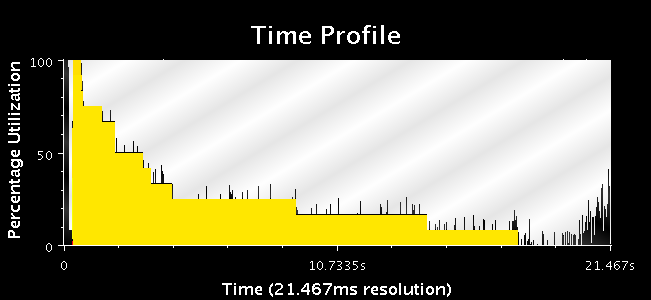
\includegraphics{1.png}
  }
& 
  \scalebox{0.35}{
    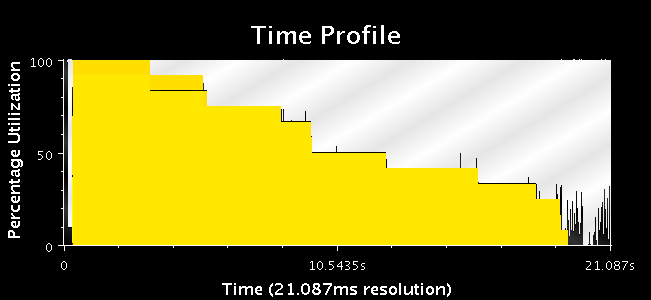
\includegraphics{2.png}
  } \\
\qquad (a) & \quad (b) \\
\end{tabular}
\caption{Percentage Utilization on graph G3 with grainsize 260, timeout = 10s   (a) Without Seed balancer (b) With ``Neighbor'' Seed Balancer}
\label{fig_sdb}
\end{figure}            

\begin{figure}
\centering
  \scalebox{0.5}{
    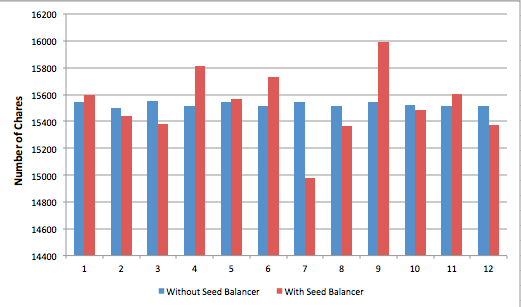
\includegraphics{3.png}
  }
\caption{Distribution of seeds on each on 12 PEs. The Seed Balancer is able is well distribute the seeds based on the PE loads. Its intutive
that PE 7 must be highly  overload so that its been given least number of seeds.}
\label{fig_chare_dist}
\end{figure}            


\section{Core Scaling}

\begin{figure}
\centering
  \scalebox{0.8}{
    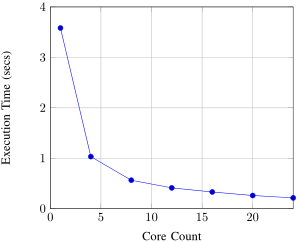
\includegraphics{core_count.png}
  }
\caption{Graph used is un-colorable G3, with 4 colors (vertices 300, Edge Density 8).  }
\label{fig_core_scale}
\end{figure}            

  For an un-colored graph all states need to be explored
  for a failure to be found and more PEs allows for a great parallelization of
    the search.
As shown  in Figure ~\ref{fig_core_scale}, the core scaling of our program was
  shown to be consistent for such graphs in the sense that more
  processors results in a smaller execution time. However, diminishing results
  are noted as the number of PEs increases, a fact that is attributed to the
  marginal reduction of time to reach a leaf node given our usage of node
  prioritization. Past a certain point the amount of work per PE to reach a
  solution containing leaf node does not decrease much as the work becomes
  adequately distributed rather quickly.  The reason for 
  


\section{Conclusion}
Our project sought to employ as many heuristics as possible to mitigate the
  exponential nature of the graph coloring problem, and this desire combined
  with experimentation of other execution parameters has allowed us to create
  an effective program for graph coloring. Many of our difficulties lay in
  fine-tuning our heuristics to work with the large variation in graph
  structure that could occur, as well as working with the non-deterministic
  effects in the exploration of the state-space tree. In the future this work
  could be expanded upon to more clearly express the impact of each heuristic
  on a graph, and to change the applications of each heuristic automatically
  depending on the characteristics of the graph. That being said, we believe we
  have provided a solid groundwork for such work to be started.

\section{References}

\nocite{*}
\bibliography{CS598_project_proposal}

\end{document}
